% Options for packages loaded elsewhere
\PassOptionsToPackage{unicode}{hyperref}
\PassOptionsToPackage{hyphens}{url}
%
\documentclass[
]{article}
\usepackage{amsmath,amssymb}
\usepackage{iftex}
\ifPDFTeX
  \usepackage[T1]{fontenc}
  \usepackage[utf8]{inputenc}
  \usepackage{textcomp} % provide euro and other symbols
\else % if luatex or xetex
  \usepackage{unicode-math} % this also loads fontspec
  \defaultfontfeatures{Scale=MatchLowercase}
  \defaultfontfeatures[\rmfamily]{Ligatures=TeX,Scale=1}
\fi
\usepackage{lmodern}
\ifPDFTeX\else
  % xetex/luatex font selection
\fi
% Use upquote if available, for straight quotes in verbatim environments
\IfFileExists{upquote.sty}{\usepackage{upquote}}{}
\IfFileExists{microtype.sty}{% use microtype if available
  \usepackage[]{microtype}
  \UseMicrotypeSet[protrusion]{basicmath} % disable protrusion for tt fonts
}{}
\makeatletter
\@ifundefined{KOMAClassName}{% if non-KOMA class
  \IfFileExists{parskip.sty}{%
    \usepackage{parskip}
  }{% else
    \setlength{\parindent}{0pt}
    \setlength{\parskip}{6pt plus 2pt minus 1pt}}
}{% if KOMA class
  \KOMAoptions{parskip=half}}
\makeatother
\usepackage{xcolor}
\usepackage{graphicx}
\makeatletter
\def\maxwidth{\ifdim\Gin@nat@width>\linewidth\linewidth\else\Gin@nat@width\fi}
\def\maxheight{\ifdim\Gin@nat@height>\textheight\textheight\else\Gin@nat@height\fi}
\makeatother
% Scale images if necessary, so that they will not overflow the page
% margins by default, and it is still possible to overwrite the defaults
% using explicit options in \includegraphics[width, height, ...]{}
\setkeys{Gin}{width=\maxwidth,height=\maxheight,keepaspectratio}
% Set default figure placement to htbp
\makeatletter
\def\fps@figure{htbp}
\makeatother
\setlength{\emergencystretch}{3em} % prevent overfull lines
\providecommand{\tightlist}{%
  \setlength{\itemsep}{0pt}\setlength{\parskip}{0pt}}
\setcounter{secnumdepth}{-\maxdimen} % remove section numbering
\ifLuaTeX
  \usepackage{selnolig}  % disable illegal ligatures
\fi
\usepackage{bookmark}
\IfFileExists{xurl.sty}{\usepackage{xurl}}{} % add URL line breaks if available
\urlstyle{same}
\hypersetup{
  hidelinks,
  pdfcreator={LaTeX via pandoc}}

\author{}
\date{}

\begin{document}

\section{信号与系统}\label{ux4fe1ux53f7ux4e0eux7cfbux7edf}

\subsection{task 1 What's the role of the Fourier transform in signals
and systems'
analysis?}\label{task-1-whats-the-role-of-the-fourier-transform-in-signals-and-systems-analysis}

从\textbf{物理意义}上说:傅里叶变换的本质是将信号从时域转换为\textbf{频域}。傅里叶变换的出现颠覆了人类对世界的认知:\textbf{世界不仅可以看作时间的变化,也可以看做各种频率不同加权的组合}。

在\textbf{通信领域},没有信号的频域分析,将很难在时域理解一个信号。因为通信领域中经常需要用\textbf{频率划分信道},所以一个信号的频域特性要比时域特性重要。贯穿时域与频域的方法之一,就是传中说的傅里叶分析。傅里叶分析可分为傅里叶级数(\emph{Fourier
Serie})和傅里叶变换(\emph{Fourier Transformation})。

傅里叶级数的本质是将一个周期的信号分解成无限多分开的(离散的)正弦波(图一),但是宇宙似乎并不是周期的。

\includegraphics{D:/Users/hehey/Documents/md/SS翻转课堂/assets/v2-38d2e076c57f6d3dd28749c77c89ed6e_b.webp}

\includegraphics{D:/Users/hehey/Documents/md/SS翻转课堂/assets/40cf849e55ed95732a60b52d4019d609_1440w.webp}

因此在信号与系统中傅里叶变换,是将一个时域非周期的连续信号,转换为一个在频域非周期的连续信号。也可以说实际上是对一个周期无限大的函数进行傅里叶变换。(图三)

\includegraphics{D:/Users/hehey/Documents/md/SS翻转课堂/assets/ece53f825c6de629befba3de12f929a7_1440w.webp}

(注:将傅里叶级数的离散频谱图无限靠近从而成为连续谱)

由一个方波信号进行分析

\includegraphics{D:/Users/hehey/Documents/md/SS翻转课堂/assets/097c9051af221c171730d4bc8f436a72_1440w.webp}

在时域中,方波信号是一个周期性的信号,由无限多的正弦波组成,频率为奇数倍的基波频率。在频域中,方波信号的频谱是一个无限多的频率分量的组合,频率为奇数倍的基波频率。这就是傅里叶变换的物理意义。傅里叶变换主要应用于波的处理

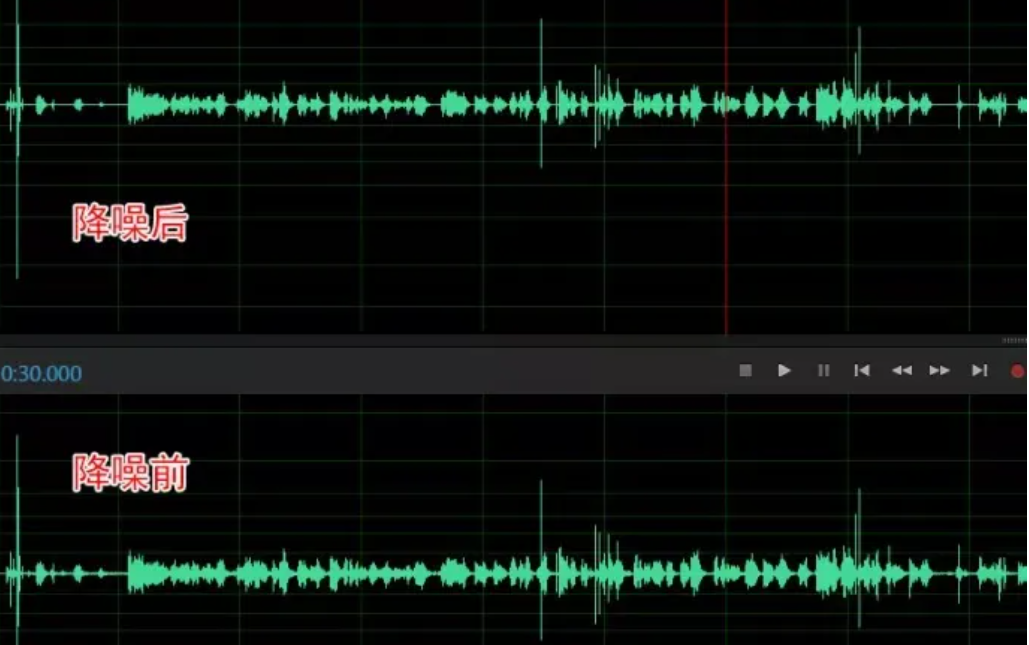
\includegraphics{D:/Users/hehey/Documents/md/SS翻转课堂/assets/屏幕截图 2024-03-24 164753.png}

图片处理

图片中大致轮廓主要由低频信号决定,细节部分由高频信号决定

人眼看到图片可以说是人脑进行的一次快速傅里叶变换
将图片分解为低频信号和高频信号

而在实际生活中图片处理如美颜相机磨皮功能等等即进行傅里叶变换对高频信号进行处理从而图片细节部分

(让我们开一下美颜=让我们开一下傅里叶变换)

\includegraphics{D:/Users/hehey/Documents/md/SS翻转课堂/assets/10050b2f27e080f59b730655923500d0_1440w.webp}

声音处理

女:高频 男:低频

随着信息时代发展
网络上随时可见变音或声音合成技术的技术,这也是一项利用傅里叶变换进行的声音处理技术

变声:

男------\textgreater 女:傅里叶变换分解---调节频率提高频率---傅里叶逆变换合成

女------\textgreater 男:傅里叶变换分解---调节频率降低频率---傅里叶逆变换合成

声音处理:

利用傅里叶变换合成想要的声音

人脑的又一次快速傅里叶变换:

在嘈杂环境下,经过迅速的傅里叶变换区分高频和低频信号,能够区分男声女声以及杂音,进行滤波来获取想听到的声音。

\subsection{task 2 For the properties of the continuous-time Fourier
transform, what does the relationship between the characteristics of
signals in time and frequency domains they
show?}\label{task-2-for-the-properties-of-the-continuous-time-fourier-transform-what-does-the-relationship-between-the-characteristics-of-signals-in-time-and-frequency-domains-they-show}

\subsubsection{4.3.0 Uniqueness
(唯一性)}\label{430-uniqueness-ux552fux4e00ux6027}

\[\mathcal{F}\{x_1(t)\}=\mathcal{F}\{x_2(t)\}  \to x_1(t)=x_2(t)\\
\mathcal{F}^{-1}\{x_1(t)\}=\mathcal{F}^{-1}\{x_2(t)\}  \to X_1(j\omega)=X_2(j\omega)\]

傅里叶变换的唯一性表明了信号及其频谱之间的一
一对应关系。这一性质给信号的变换、处理、鉴别
和恢复提供了理论依据。如:气体检测、矿物鉴定。

\subsubsection{4.3.1 Linearity (线性)}\label{431-linearity-ux7ebfux6027}

if:

\[x(t)\stackrel{\mathcal{F}}{\longleftrightarrow}X(j\omega),   y(t)\stackrel{\mathcal{F}}{\longleftrightarrow} Y(j\omega)\\\]

then:

\[ax(t)+by(t)\stackrel{\mathcal{F}}{\longleftrightarrow}aX(j\omega)+bY(j\omega)\]

\subsubsection{4.3.2 时移性质}\label{432-ux65f6ux79fbux6027ux8d28}

若:

\[x(t)\stackrel{\mathcal{F}}{\longleftrightarrow}X(j\omega)\]

则有:

\[x(t-t_0)\stackrel{\mathcal{F}}{\longleftrightarrow}e^{-j\omega t_0}X(j\omega)\]

证明:

\[x(t)=\frac{1}{2\pi}\int_{-\infty}^{+\infty}X(j\omega)e^{j\omega t}d\omega\]

在该式中以 \(t-t_0\) 取代t,可得

\[x(t-t_0)=\frac{1}{2\pi}\int_{-\infty}^{+\infty}X(j\omega)e^{j\omega (t-t_0)}d\omega\\
=\frac{1}{2\pi}\int_{-\infty}^{+\infty}(e^{-j\omega t_0 }X(j\omega))e^{j\omega t}d\omega\]

所以可得:

\[\mathcal{F}\{x(t-t_0)\} =e^{-j\omega t_0}X(j\omega)\]

Time Shift \( \Longleftrightarrow \) Phase Shift (时域平移
\( \Longleftrightarrow \) 频域相移)

\[X(j\omega)e^{-j\omega t_0}=|X(j\omega)|e^{j[\varphi(j\omega)-\omega t_0]}\]

对\(\omega\)频率分量,幅度密度没变,相位改变为:

\[\Delta\varphi = -\omega t_0\]

\subsubsection{4.3.3
共轭与共轭对称性质}\label{433-ux5171ux8f6dux4e0eux5171ux8f6dux5bf9ux79f0ux6027ux8d28}

共轭性质是指,若:

\[x(t)\stackrel{\mathcal{F}}{\longleftrightarrow}X({j\omega})\]

则有:

\[x^*(t)\stackrel{\mathcal{F}}{\longleftrightarrow}X^*(j\omega)\]

证明:

\[X^*(j\omega) = [\int_{-\infty}^{+\infty}x(t)e^{-j\omega t}dt]^*\\
=\int_{-\infty}^{+\infty}x^*(t)e^{j\omega t}dt\]

用\(-\omega\)代替\(\omega\),可得:

\[X^*(-j\omega)=\int_{{-\infty}}^{+\infty}x^*(t)e^{-j\omega t}dt\]

特别的,如果\&x(t)\&是实函数,则\(X(j\omega)\)具有共轭对称性:

\[X(-j\omega)=X^*(j\omega)\]

具有共轭对称性的函数在数学上称为厄米函数 (Hermitian function)

厄米函数(Hermitian function)定义为:

\[f(-x)=f^*(x)\]

其波形对称性表现为:实部偶函数、虚部奇函数

\[Re\{X(j\omega)\}=Re\{X(-j\omega)\}\\
Im\{X(j\omega)\}=-Im\{X(-j\omega)\}\]

FT共轭对称性:实信号的傅氏变换是厄米函数

实信号频谱对称性:

\[\left\{
\begin{aligned}
    |X(j\omega|&=\sqrt{Re(\omega)^2+Im(\omega)^2}\\
    \varphi(j\omega)&=arctan{\frac{Im(\omega)}{Re(\omega)}}
\end{aligned}
\right.\]

\subsubsection{4.3.4
微分与积分性质}\label{434-ux5faeux5206ux4e0eux79efux5206ux6027ux8d28}

\[x(t)=\frac{1}{2\pi}\int_{-\infty}^{+\infty}X(j\omega)e^{j\omega t}d\omega\]

将上式两边对t微分:

\[\frac{dx(t)}{dt}=\frac{1}{2\pi}\int_{-\infty}^{+\infty}j\omega X(j\omega)e^{j\omega t}d\omega\]

因此有:

\[\frac{dx(t)}{dt}\stackrel{\mathcal{F}}{\longleftrightarrow}j\omega X(j\omega)\]

从而微分性质:

\[x^{(n)}(t)\stackrel{\mathcal{F}}{\longleftrightarrow}(j\omega)^nX(j\omega)\\
X^{(n)}(j\omega)\stackrel{\mathcal{F}}{\longleftrightarrow}(-jt)^nx(t)\]

积分性质:

\[\int_{-\infty}^tx(\tau)d\tau\stackrel{\mathcal{F}}{\longleftrightarrow}\frac{1}{j\omega}X(j\omega)+\pi X(0)\delta (\omega)\\
\mathcal F\{u(t)\}=\int_{-\infty}^t\delta(\tau)d\tau = \frac{1}{j\omega}+\pi\delta(\omega)\]

\subsubsection{4.3.5
时间与频率的尺度变换性质}\label{435-ux65f6ux95f4ux4e0eux9891ux7387ux7684ux5c3aux5ea6ux53d8ux6362ux6027ux8d28}

若:

\[x(t)\stackrel{\mathcal{F}}{\longleftrightarrow}X(j\omega)\]

则有:

\[x(at)\stackrel{\mathcal{F}}{\longleftrightarrow}\frac{1}{|a|}X(\frac{j\omega}{a})\\
\frac{1}{|b|}x(\frac{t}{b})\stackrel{\mathcal{F}}{\longleftrightarrow}X(jb\omega)\]

其中,a是常实数。这个性质可直接由傅里叶变换的定义得到(只写了第一个式子):

\[\mathcal F\{x(at)\}=\int_{-\infty}^{+\infty}x(at)e^{-j\omega t}dt\]

利用\(\tau=at\),替换后可得:

\[\mathcal F\{x(at)\}=
\left\{
\begin{aligned}
    \frac{1}{a}\int_{-\infty}^{+\infty}x(\tau)e^{-j(\omega/a)\tau d\tau} ,  && a>0\\
    -\frac{1}{a}\int_{-\infty}^{+\infty}x(\tau)e^{-j(\omega/a)\tau d\tau}, &&a<0
\end{aligned}
\right.\]

时域中波形压缩(扩展)\(\to\)频域中波形扩展(压缩)

特别地,当a=-1时:

\[x(-t)\stackrel{\mathcal{F}}{\longleftrightarrow}X(-j\omega)\]

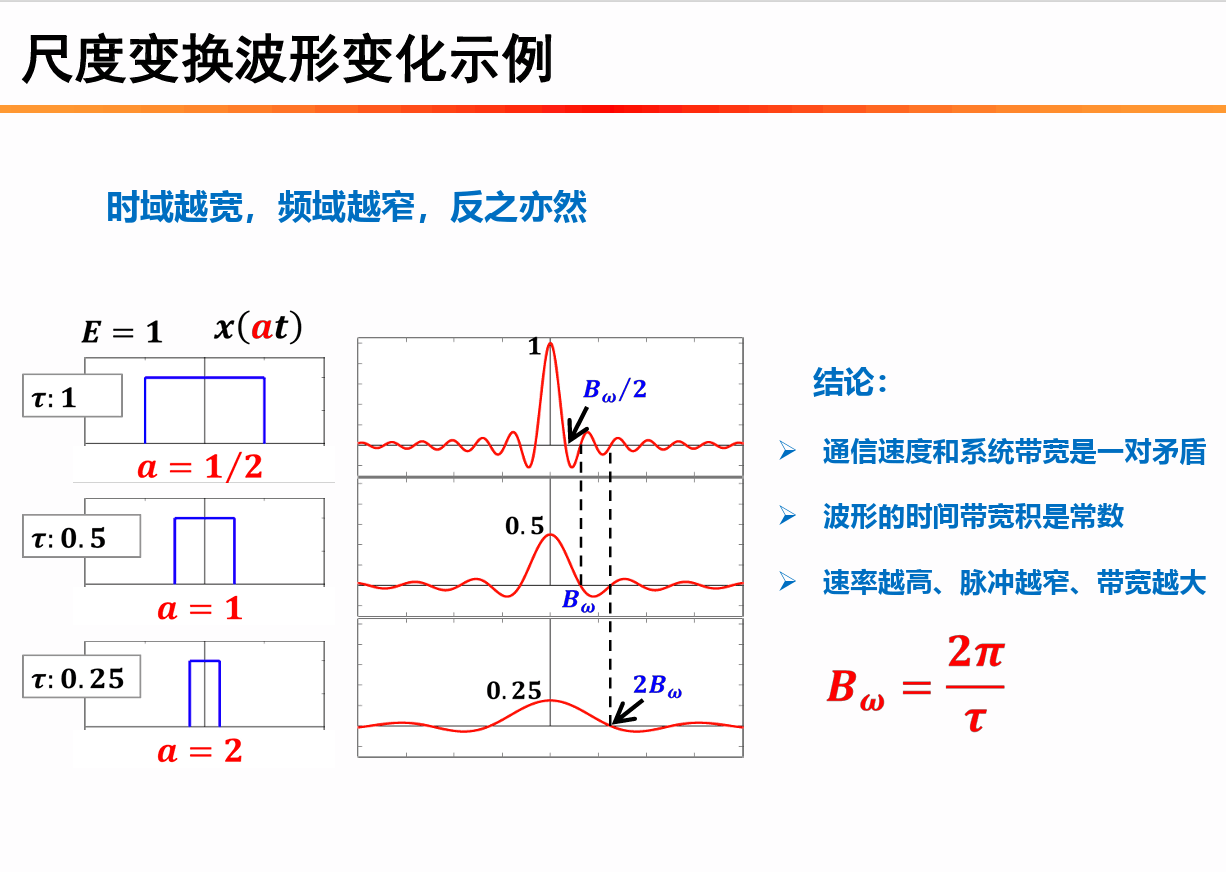
\includegraphics{D:/Users/hehey/Documents/md/SS翻转课堂/assets/b37bc84492e5a277fb5e8352405fc0b9.png}

\subsubsection{4.3.6 对偶性质}\label{436-ux5bf9ux5076ux6027ux8d28}

if:

\[x(t)\stackrel{\mathcal{F}}{\longleftrightarrow}X(\omega)\]

then:

\[X(t)\stackrel{\mathcal{F}}{\longleftrightarrow}2\pi x(-\omega)\\

\left\{

\begin{aligned}

    X(t)=X(\omega)|_{\omega = t}\\

    x(\omega)=x(t)|_{t=\omega}

\end{aligned}

\right.\\

x(t)=\frac{1}{2\pi}\int_{-\infty}^{\infty}X(\omega)e^{j\omega t}d\omega\\

x(-t)=\frac{1}{2\pi}\int_{-\infty}^{\infty}X(\omega)e^{-j\omega t}d\omega\\

x(-\omega)=\frac{1}{2\pi}\int_{-\infty}^{\infty}X(t)e^{-j\omega t}dt\\

\to 2\pi x(-\omega)=\int_{-\infty}^{\infty}X(t)e^{-j\omega t}dt = \mathcal F\{X(t)\}\]

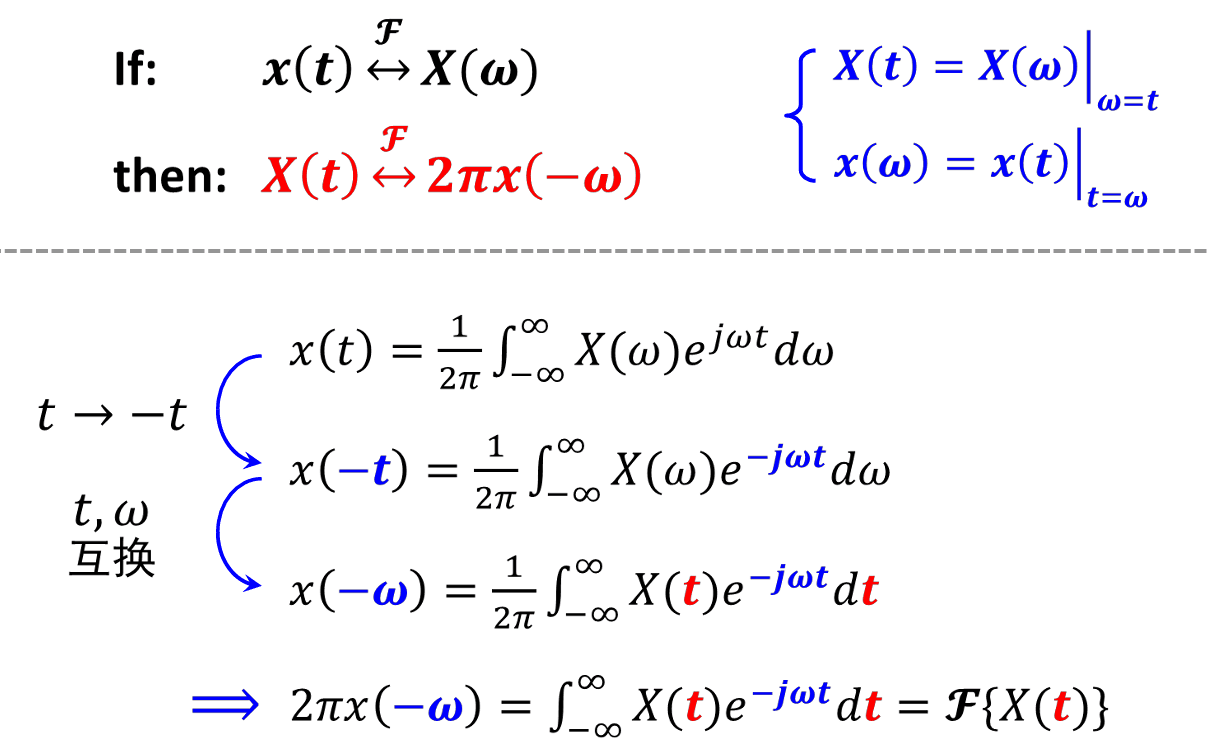
\includegraphics{D:/Users/hehey/Documents/md/SS翻转课堂/assets/e29a821d9b891c6360daae94bad52363.png}

时域和频域波形可互换:波形变化规律保持不变

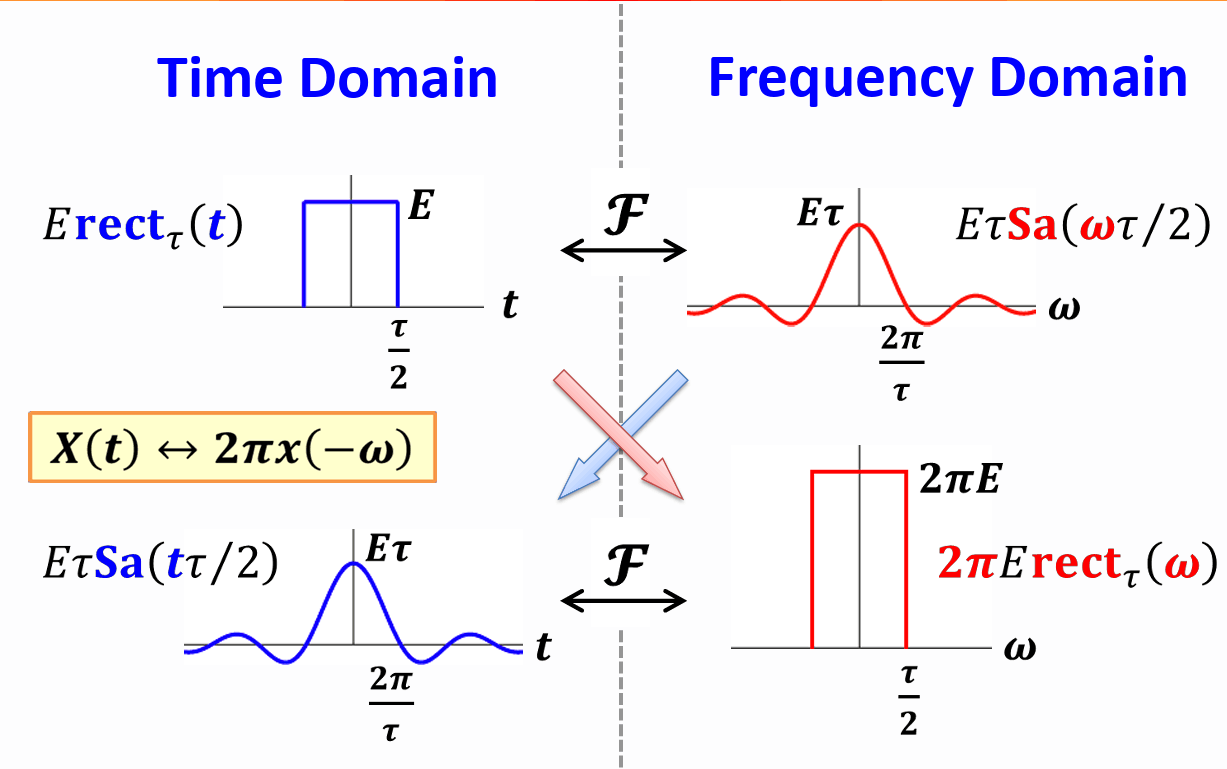
\includegraphics{D:/Users/hehey/Documents/md/SS翻转课堂/assets/62b5124657211c37d7e760236ffb8861.png}

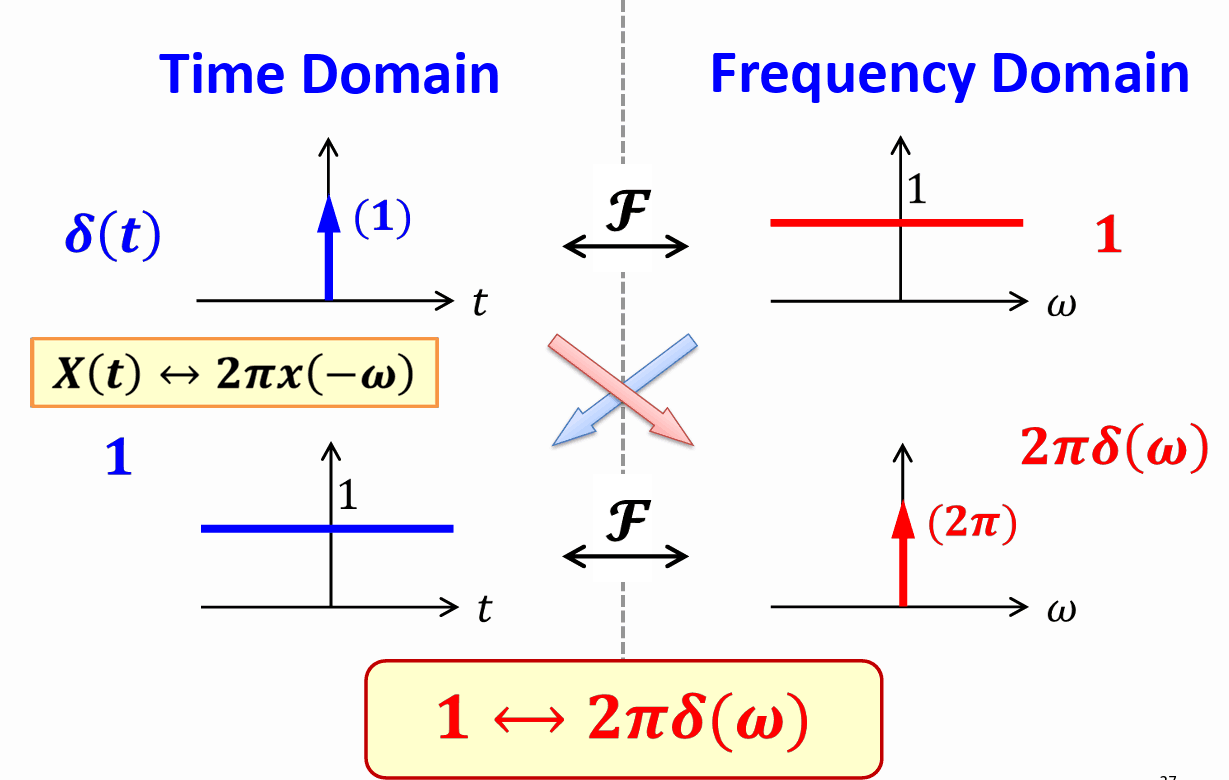
\includegraphics{D:/Users/hehey/Documents/md/SS翻转课堂/assets/80e8fdc4df2327e9d2c79eeb2cb36e7b.png}

\subsubsection{4.3.7
帕塞瓦尔定理}\label{437-ux5e15ux585eux74e6ux5c14ux5b9aux7406}

若:

\[x(t)\stackrel{\mathcal{F}}{\longleftrightarrow}X(j\omega)\]

则有:

\[\int_{-\infty}^{+\infty}|x(t)|^2dt=\frac{1}{2\pi}\int_{-\infty}^{+\infty}|X(j\omega)|^2d\omega\]

前提:x(t)时能量(有限)信号

证明:

\[\int_{-\infty}^{+\infty}|x(t)|^2dt=\int_{-\infty}^{+\infty}x(t)\bar{x(t)}dt\\
=\int_{-\infty}^{+\infty}x(t)[\frac{1}{2\pi}\int_{-\infty}^{+\infty}\bar{X(j\omega)}e^{-j\omega t}d\omega]dt\]

改变一下积分次序,有:

\[\int_{-\infty}^{+\infty}|x(t)|^2dt = \frac{1}{2\pi}\int_{-\infty}^{+\infty}X^*(j\omega)[\int_{-\infty}^{+\infty}x(t)e^{-j\omega t}dt]d\omega\]

因此可以得到:

\[\int_{-\infty}^{+\infty}|x(t)|^2dt=\frac{1}{2\pi}\int_{-\infty}^{+\infty}|X(j\omega)|^2d\omega\]

\subsection{task 3 Is there a continuous-time signal which has an
infinite frequency
band-width?}\label{task-3-is-there-a-continuous-time-signal-which-has-an-infinite-frequency-band-width}

\subsection{task 4 In some cases, even if a continuous-time signal does
not satisfy the condition of absolutely integrable* we still can find
its Fourier transform. Can you list some of this kind of signals? And
How to find their Fourier
transform?}\label{task-4-in-some-cases-even-if-a-continuous-time-signal-does-not-satisfy-the-condition-of-absolutely-integrable-we-still-can-find-its-fourier-transform-can-you-list-some-of-this-kind-of-signals-and-how-to-find-their-fourier-transform}

\subsection{\texorpdfstring{task 5 For signals 𝑥(𝑡) = 𝑢(𝑡 + 1) − 𝑢(𝑡 −
1) and\(y(t)=\sum^{+\infty}_{k=-\infty}[u(t+1-5k)-u(t-1-5k)]\),how the
Fourier transform of 𝑥𝑥(𝑡𝑡) relates to that of 𝑦𝑦(𝑡𝑡)?
Explain.}{task 5 For signals 𝑥(𝑡) = 𝑢(𝑡 + 1) − 𝑢(𝑡 − 1) andy(t)=\textbackslash sum\^{}\{+\textbackslash infty\}\_\{k=-\textbackslash infty\}{[}u(t+1-5k)-u(t-1-5k){]},how the Fourier transform of 𝑥𝑥(𝑡𝑡) relates to that of 𝑦𝑦(𝑡𝑡)? Explain.}}\label{task-5-for-signals-ux1d465ux1d461--ux1d462ux1d461--1-ux2212-ux1d462ux1d461-ux2212-1-and-ux1d466--ux1d461---ux2211-ux1d458--ux2212-ux221e--ux221e--ux1d462--ux1d461--1-ux2212-5-ux1d458--ux2212-ux1d462--ux1d461-ux2212-1-ux2212-5-ux1d458---how-the-fourier-transform-of-ux1d465ux1d465ux1d461ux1d461-relates-to-that-of-ux1d466ux1d466ux1d461ux1d461-explain}

\begin{aligned}

x(t) & =u(t+1)-u(t-1) \\

y(t) & =\sum_{k=-\infty}^{\infty} x(t-5 k) \\

x(t) \leftrightarrow f(x(t)) & =\int_{-1}^{1} e^{j w t} d t=\frac{1}{-j w}\left(e^{-j w}-e^{j w}\right) \\

y(t) \leftrightarrow f(y(t)) & =\sum_{k=-\infty}^{\infty} \int_{5 k-1}^{5 k+1} e^{-j w t} d t \\

& =\sum_{k=-\infty}^{\infty} \frac{1}{-j w}\left[e^{-j w(5 k+1)}-e^{-j w(5 k+1)}\right] \\

& =\sum_{k=-\infty}^{\infty} \frac{e^{j w 5 k}}{-j w}\left(e^{-j w}-e^{j w}\right) \\

& =\sum_{k=-\infty}^{\infty} e^{-j w 5 k} \cdot f(x(t))

\end{aligned}

\subsection{task 6 For signals 𝑥𝑥(𝑡𝑡) = 𝑢(𝑡 + 0.5) − 𝑢(𝑡 − 0.5) and 𝑦(𝑡)
= (1 + cosπ𝑡){[}𝑢(𝑡 + 0.5) −𝑢(𝑡 − 0.5){]}, which of them is smoother?
You can find answer after you obtain their magnitude
spectra.}\label{task-6--for-signals-ux1d465ux1d465ux1d461ux1d461--ux1d462ux1d461--05-ux2212-ux1d462ux1d461-ux2212-05-and-ux1d466ux1d461--1--cosux3c0ux1d461ux1d462ux1d461--05-ux2212ux1d462ux1d461-ux2212-05-which-of-them-is-smoother-you-can-find-answer-after-you-obtain-their-magnitude-spectra}

\subsection{task 7 How to use Fourier transform to determine the
response 𝑦(𝑡) for a continuous-time LTI system to an input signal
𝑥(𝑡)?}\label{task-7-how-to-use-fourier-transform-to-determine-the-response-ux1d466ux1d461-for-a-continuous-time-lti-system-to-an-input-signal-ux1d465ux1d461}

下面是使用傅里叶变换来确定连续时间 LTI 系统对输入信号 x(t)的响应
y(t)的一般步骤:

\begin{enumerate}
\def\labelenumi{\arabic{enumi}.}
\item
  对输入信号 x(t)进行傅里叶变换,得到 X(jω)。
\item
  根据 LTI 系统的频率响应 H(jω),计算输出信号的傅里叶变换 Y(jω)。
\item
  对 Y(jω)进行傅里叶逆变换,得到输出信号 y(t)。
\end{enumerate}

数学概念或定理:傅里叶变换是一种将时域信号转换为频域信号的数学工具。对于连续时间信号
x(t),它的傅里叶变换 X(jω)表示信号在不同频率 ω
处的频谱分量。同样,傅里叶逆变换将频域信号转换回时域信号。

解题步骤:

\begin{enumerate}
\def\labelenumi{\arabic{enumi}.}
\item
  对输入信号 x(t)进行傅里叶变换:X(jω) = ∫x(t)e\^{}\{-jωt\}dt
\item
  根据 LTI 系统的频率响应 H(jω),计算输出信号的傅里叶变换:Y(jω) =
  H(jω)X(jω)
\item
  对 Y(jω)进行傅里叶逆变换,得到输出信号
  y(t):\(y(t) = \int Y(j\omega)e^{j\omega t}d\omega\)
\end{enumerate}

需要注意的是,在实际应用中,可能需要考虑一些具体的条件和限制,例如信号的边界条件、系统的稳定性等。

\subsection{task 8 What are frequency selective filters? Why do we
explore ideal frequency selective filters? Why are ideal filters
unrealizable?}\label{task-8-what-are-frequency-selective-filters-why-do-we-explore-ideal-frequency-selective-filters-why-are-ideal-filters-unrealizable}

\subsection{task 9 Can you relate Fourier Transform with one of Chairman
Xi's words (points of view)
?}\label{task-9-can-you-relate-fourier-transform-with-one-of-chairman-xis-words-points-of-view-}

傅里叶的核心思想概括起来有以下两条.

(1)\textsuperscript{1}任何一个复杂的函数(或描述事物变化的
物理量)在一定的条件下都可以分解为许多简单的
正弦或余弦函数的和.具体内容有以下4条.

\begin{itemize}
\item
  任何一个周期函数(在满足所谓的``狄利克
  雷或狄里希利条件''下)均可以看成无穷多个(频率 跃变的)正(余)弦函数之和.
\item
  任何一个定义在有限区域上的非周期函数,
  均可以通过``延拓''的方法把它转化为周期函数,从 而仍然 可 以 把 它 看 成
  无 穷 多 个 (频 率 跃 变 的)正 (余)弦函数的叠加.
\item
  任何一个(定义在无限区域上的)非周期函
  数,都可以看成无穷多个频率连续变化的正(余)弦 函数的和(积分).
\item
  定义在无限小空间区域(即一个点)上的非 周期函数(即所谓的δ
  函数),可以看成无穷多个频 率连续变化的正(余)弦函数的和(积分).
\end{itemize}

习近平新时代中国特色社会主义思想的核心内容可以概括为``十个明确''和``十四个坚持''。这些内容体现了习近平总书记对中国特色社会主义建设规律的深化认识和理论创新的重大成果。具体包括:

\begin{itemize}
\item
  \textbf{``十个明确''}:

  \begin{enumerate}
  \def\labelenumi{\arabic{enumi}.}
  \item
    明确中国特色社会主义最本质的特征是中国共产党领导。
  \item
    明确坚持和发展中国特色社会主义的总任务是实现社会主义现代化和中华民族伟大复兴。
  \item
    明确新时代我国社会主要矛盾是人民日益增长的美好生活需要和不平衡不充分的发展之间的矛盾。
  \item
    明确中国特色社会主义事业总体布局是``五位一体'',战略布局是``四个全面''。
  \item
    明确全面深化改革的总目标是完善和发展中国特色社会主义制度、推进国家治理体系和治理能力现代化。
  \item
    明确全面推进依法治国的总目标是建设中国特色社会主义法治体系、建设社会主义法治国家。
  \item
    明确必须坚持和完善社会主义基本经济制度,使市场在资源配置中起决定性作用。
  \item
    明确党在新时代的强军目标是建设一支听党指挥、能打胜仗、作风优良的人民军队。
  \item
    明确中国特色大国外交要服务民族复兴、促进人类进步。
  \item
    明确全面从严治党的战略方针。
  \end{enumerate}
\item
  \textbf{``十四个坚持''}:

  \begin{enumerate}
  \def\labelenumi{\arabic{enumi}.}
  \item
    坚持党对一切工作的领导。
  \item
    坚持以人民为中心。
  \item
    坚持全面深化改革。
  \item
    坚持新发展理念。
  \item
    坚持人民当家作主。
  \item
    坚持全面依法治国。
  \item
    坚持社会主义核心价值体系。
  \item
    坚持在发展中保障和改善民生。
  \item
    坚持人与自然和谐共生。
  \item
    坚持总体国家安全观。
  \item
    坚持党对人民军队的绝对领导。
  \item
    坚持``一国两制''和推进祖国统一。
  \item
    坚持推动构建人类命运共同体。
  \item
    坚持全面从严治党。
  \end{enumerate}
\end{itemize}

傅里叶和习主席的观点的共同点是都是对一个系统的规律性的认识,傅里叶是对物理世界的规律性的认识,习主席是对社会主义建设规律的认识。他们都是通过对系统的分析和研究,提出了一系列的理论和观点,从而指导实践,推动事业的发展。他们的观点都是基于对事物本质的深刻理解和对规律性的把握,体现了对科学和实践的不懈追求。他们的观点都是为了实现人类社会的和谐与进步,为了实现人类的共同发展和繁荣。

傅里叶首先是一个物理学家,他在求解热传导方程时,创立了一套数学理论(核心即傅里叶变换),解决了一类偏微分方程的定解问题.这一点和习主席颇为相似.习主席在谈论治国理政时时,提出了一系列治国理政新理念新思想新战略,实现了实践创新、理论创新、制度创新、文化创新以及各方面创新,形成了系统完整、逻辑严密的科学理论体系。\textsuperscript{2}在此基础上创造性地回答了``五大问题'',进一步深化了对``五大规律''的认识.但是,他们两个的面对的问题不同,思维方式也是不同的.

傅里叶和习主席虽然在他们的领域有着卓越的成就和独特的贡献,但他们面临的问题和思维方式却截然不同。

傅里叶作为物理学家,他的思维方式是基于实验和数学模型的。他通过观察和实验,发现了热传导的规律,并尝试用数学语言来描述这一规律。傅里叶变换的核心在于将一个复杂的问题分解为简单的组成部分,通过对每个组成部分进行分析和处理,最后再将其组合起来,从而得到整个问题的解。这种思维方式体现了傅里叶对物理世界的深刻理解和精确把握。

而习主席作为一位政治家,他的思维方式则更加注重实践和创新。他通过对中国国情的深入分析和对国内外形势的敏锐洞察,提出了一系列治国理政新理念新思想新战略。这些理念、思想和战略不仅具有理论价值,更重要的是能够指导实践,推动中国的改革开放和现代化建设。习主席的思维方式体现了对中国发展的深刻思考和大胆创新。

尽管傅里叶和习主席面临的问题和思维方式不同,但他们都展现出了对科学、实践和创新的不懈追求。他们通过自己的努力和智慧,为人类社会的进步和发展做出了卓越的贡献。他们的故事和成就,不仅为我们提供了宝贵的经验和启示,也激励着我们不断前行,探索未知,创造未来。

页尾

参考文献

\begin{enumerate}
\def\labelenumi{\arabic{enumi}.}
\item
  蔡志东.物理通报.傅里叶思想的精髓及其伟大之处.2021.4
\item
  姜 辉.红旗文稿2017/13.习近平治国理政思想的理论贡献
\end{enumerate}

\subsection{task 10 Music synthesis and Sound
processing(音乐合成与音效处理)}\label{task-10-music-synthesis-and-sound-processingux97f3ux4e50ux5408ux6210ux4e0eux97f3ux6548ux5904ux7406uxff09}

In music synthesis, the Fourier transform is used to analyze and
synthesize sounds. For example, in a synthesizer, we can use the Fourier
transform to decompose a complex musical signal into a series of sine or
cosine waves that represent components of different frequencies in the
musical signal. We can then resynthesize entirely new sounds by
adjusting the amplitude, frequency, and phase of these waves.
(在音乐合成中,傅里叶变换被用来分析和合成声音。例如,在合成器中,我们可以使用傅里叶变换将一段复杂的音乐信号分解为一系列正弦波或余弦波,这些波代表了音乐信号中不同频率的成分。然后,我们可以通过调整这些波的振幅、频率和相位,重新合成出全新的声音。)

In sound effects processing. When we record an audio, we may be
disturbed by ambient noise, such as wind sound, electric current sound,
etc. These noises often contain many highfrequency components. Through
the Fourier transform, we can identify these high-frequency noise
components and filter them in the frequency domain to remove them.
(在音效处理中。当我们录制一段音频时,可能会受到环境噪声的干扰,比如风声、电流声等。这噪声通常包含许多高频成分。通过傅里叶变换,我们可以将这些高频噪声成分识别出来,并在频域中进行滤波,从而去除这些噪声。)

\end{document}
